\documentclass{mnras}
\usepackage{graphicx}
\usepackage{amsmath}
\usepackage{natbib}
\usepackage{hyperref}

\title[Density Profile of Merged Dark Matter Remnant]{Density Profile of the Merged Dark Matter Remnant}
\author[Zach Harnist]{Zach\\Department of Astronomy, University of Arizona}
\date{March 20, 2025}

\begin{document}

\maketitle

\begin{abstract}
Dark matter (DM) halo mergers play a key role in the formation of hierarchical structures. 
This proposal outlines my plan to investigate the density profile of the remnant halo formed by the Milky Way's (MW) and Andromeda's (M31) massive merger. 
I will ascertain how the density structure changes after the merger by using theoretical models like the Navarro-Frenk-White (NFW) and Hernquist profiles as well as numerical simulations. 
I think that dynamical relaxation may lead the core density to drop while the overall profile maintains its cuspy appearance. 
My work will advance our knowledge of how cosmic structures are formed and how galaxy-scale DM structures react to massive mergers.
\end{abstract}

\begin{keywords}
cosmology: dark matter -- galaxies: halos -- galaxies: evolution -- methods: numerical
\end{keywords}

\section{Introduction}

Galaxies' gravitational backbone is made up of dark matter halos, which have an impact on their structure and development. Small halos may combine over cosmic time to generate larger formations, according to the hierarchical merging process anticipated by $\Lambda$CDM cosmology. A rare opportunity to investigate how such significant interactions alter dark matter distributions is presented by the MW and M31's upcoming merger. In this study, I will measure the combined halo remnant's density profile and assess if it fits well-known theoretical models like the Hernquist or NFW profiles.

Galaxy evolution depends on our ability to comprehend the density distribution of dark matter halos. The distribution of baryonic matter, satellite galaxy formation, and star motion are all influenced by the halo's concentration and shape. Mergers can cause mass redistribution according to previous research, which might change the density profile and perhaps change the inner slope \citep[Frenk \& White 2012]{Frenk2012}, \citep[Abadi et al. 2010]{Abadi2010}. Whether these modifications bring major deviations from classical models or follow a predictable pattern is unclear, though \citep[Drakos et al. 2019a]{Drakos2019a}, \citep[Drakos et al. 2019b]{Drakos2019b}. In order to determine how well current models capture the ensuing halo, my research will examine the post-merger density structure.

Numerical simulations suggest that major mergers may flatten central density cusps, increase the scale radius, or induce density fluctuations within the remnant halo \citep[Prada 2019]{Prada2019}. These processes occur due to violent relaxation, which redistributes energy and alters particle orbits. Figure \ref{fig:density_evolution} illustrates how dark matter density evolves through various stages of a major merger, highlighting the redistribution of mass, central cusp flattening, and halo relaxation processes that my study aims to characterize quantitatively.

\begin{figure}
    \centering
    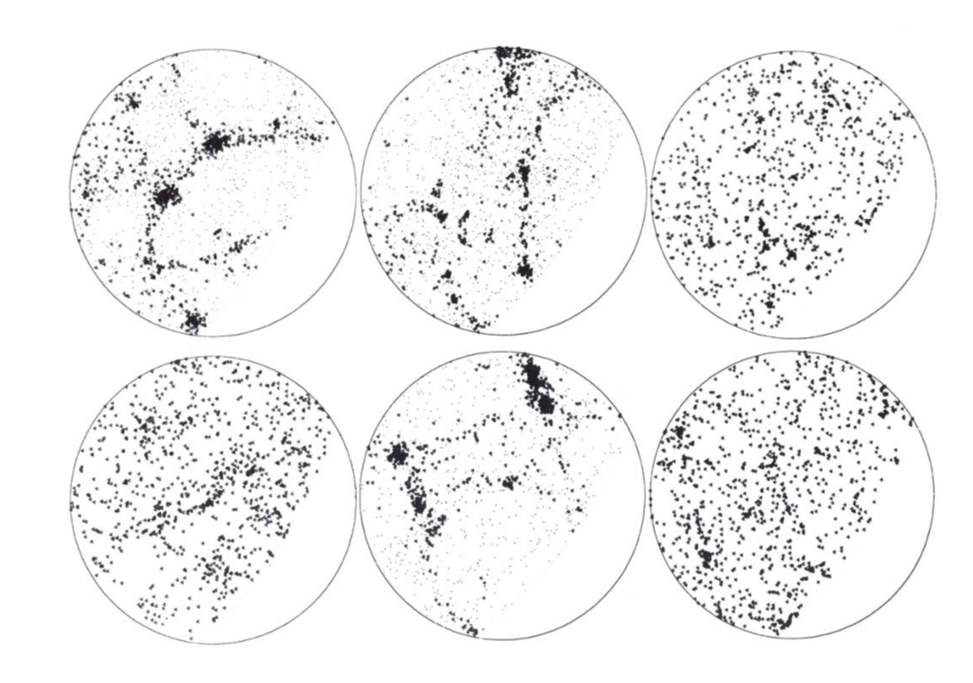
\includegraphics[width=0.8\linewidth]{density_profile.png}
    \caption{Dark matter halo evolution over time, showing how major mergers and relaxation processes affect the density structure of the remnant halo. Each panel represents a different merger stage, illustrating the redistribution of mass and the formation of the final density profile. This visualization provides insight into the transformation of the dark matter distribution during the MW-M31 merger. Adapted from Navarro et al. (1997).}
    \label{fig:density_evolution}
\end{figure}

\section{Methods}

To answer the research question regarding how the merged dark matter halo compares to the Hernquist profile, I will conduct an analysis of cosmological simulations that model the MW-M31 major merger. I will compute radial density profiles by binning dark matter particles in spherical shells, using a logarithmic spacing to capture both inner and outer halo regions effectively. Density will be computed as a function of radius and compared across multiple merger snapshots, spanning before, during, and after collision.

The dark matter halo density profile will be extracted from high-resolution N-body simulations, using either pre-existing datasets or newly generated merger simulations. Data analysis will be conducted using Python, leveraging NumPy for binning, Matplotlib for visualization, and SciPy for profile fitting. 

Because the Hernquist profile can explain dark matter structures with a more centrally concentrated profile, it is frequently compared to the NFW model. The Hernquist profile has a stronger central slope of $\rho \propto r^{-1}$ but transitions more smoothly to an outer profile of $\rho \propto r^{-4}$, whereas the NFW profile has a density slope of $\rho \propto r^{-1}$ in the inner area. By comparing these two models, it will be possible to ascertain whether mass mixing and relaxation cause the post-merger halo to shift toward a changed distribution or preserve a profile closer to its progenitors.

Figure \ref{fig:method_diagram} illustrates the theoretical underpinning of how differences in dark matter particle properties (CDM, WDM, HDM) impact the formation and evolution of halo structures. These theoretical variations set expectations for interpreting deviations observed in the radial density profiles computed from the MW-M31 merger simulations.

\begin{figure}
    \centering
    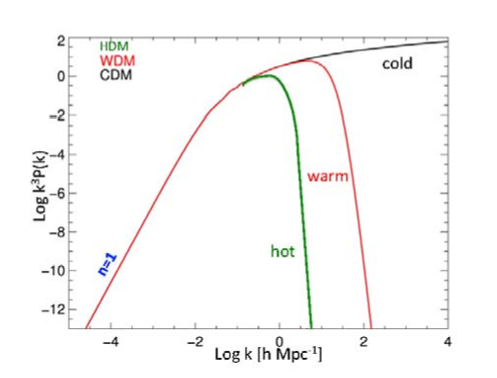
\includegraphics[width=0.8\linewidth]{figure1.png}
    \caption{Theoretical dark matter power spectrum comparison for Cold Dark Matter (CDM), Warm Dark Matter (WDM), and Hot Dark Matter (HDM). The log-log plot shows the scale-dependence of density fluctuations for different DM scenarios, which influences halo formation and structure. Understanding these differences provides essential context for interpreting possible deviations in density profiles following the MW-M31 major merger. Adapted from Frenk \& White (2012).}
    \label{fig:method_diagram}
\end{figure}

\section{Future Considerations}

There are still more general unanswered questions about the evolution of dark matter halos after significant mergers, even while my focus is on the comparison of the post-merger halo to the Hernquist profile:
\begin{enumerate}
    \item Beyond conventional theoretical models, how does the merged halo's density profile compare to that of its progenitors?
    How does the ultimate density structure get shaped by violent relaxation?
    How much does the post-merger profile change as a result of external influences like baryonic feedback and satellite interactions?
    \item Is the post-merger structure entirely explicable by normal dark matter models, or do changes need to be made?
\end{enumerate}
These more general questions offer a foundation for understanding the significance of this research in the context of dark matter halo evolution, even if I won't be directly responding to them.

\section{Hypothesis and Expected Results}

Because of mass redistribution, I predict that the merged halo will roughly follow an NFW profile, except with a somewhat larger scale radius. During the merger process, energy relaxation may cause the central density to drop, which could result in a slight departure from typical profile predictions. I anticipate that the outer density slope will continue to be in line with theoretical predictions, suggesting that mass redistribution mostly takes place in the interior regions.

I will investigate other elements like dynamical friction, baryonic feedback, or continuous accretion if the final density profile differs noticeably from theoretical predictions. I will evaluate the robustness of my findings and ascertain whether structural changes are predominantly caused by secondary astrophysical processes or gravitational interactions by examining variations.

\bibliographystyle{mnras}
\bibliography{references}

\end{document}

